%%%%%%%%%%%%%%%%%%%%%%%%%%%%%%%%%%%%%%%%%%%%%%%%%%%%%%%%%%%%
%%% ELIFE ARTICLE TEMPLATE
%%%%%%%%%%%%%%%%%%%%%%%%%%%%%%%%%%%%%%%%%%%%%%%%%%%%%%%%%%%%
%%% PREAMBLE 
\documentclass[9pt]{NEU560-final}
% Use the onehalfspacing option for 1.5 line spacing
% Use the doublespacing option for 2.0 line spacing
% Please note that these options may affect formatting.
% Additionally, the use of the \newcommand function should be limited.

\usepackage[version=4]{mhchem}
\usepackage{array,multirow}
\usepackage{hyperref}
\usepackage{graphicx}
\usepackage[parfill]{parskip}
\usepackage{siunitx}
\DeclareSIUnit\Molar{M}

%%%%%%%%%%%%%%%%%%%%%%%%%%%%%%%%%%%%%%%%%%%%%%%%%%%%%%%%%%%%
%%% ARTICLE SETUP
%%%%%%%%%%%%%%%%%%%%%%%%%%%%%%%%%%%%%%%%%%%%%%%%%%%%%%%%%%%%

\title{Matrix Normal Models for fMRI Analysis with Spatial Priors}
\author[1]{Sam Zorowitz}

%%%%%%%%%%%%%%%%%%%%%%%%%%%%%%%%%%%%%%%%%%%%%%%%%%%%%%%%%%%%
%%% ARTICLE START
%%%%%%%%%%%%%%%%%%%%%%%%%%%%%%%%%%%%%%%%%%%%%%%%%%%%%%%%%%%%

\begin{document}

\maketitle

\begin{abstract}
Conventional fMRI analysis includes spatial smoothing of the data to improve the signal-to-noise ratio. In the absence of knowledge about the spatial extent of the signal of interest, it is difficult to decide by how much to smooth the data. Here we propose a data-driven method for smoothing using matrix-normal models with spatial priors. Using both simulated and empirical data, we show the matrix-normal independent autoregressive (MN-IAR) model successfully navigates the estimation/detection power trade-off, preserving signal amplitude information while reducing noise. We also discuss the utility of the matrix-normal framework more broadly for the flexible modeling of fMRI data.
\end{abstract}

\section{Introduction}
Functional magnetic resonance imaging (fMRI) is a noninvasive tool for measuring neural activity (Poldrack et al., 2011). From measuring changes in the blood oxygenated level dependent (BOLD) signal, we can infer changes in the activity of neural populations in response to experimental events-of-interest. We denote a single fMRI timeseries dataset as $Y \in \mathbb{R}^{T,V}$, where $T$ is the number of time points (acquisitions) and $V$ is the number of voxels. In conventional fMRI analysis, the dataset is modeled linearly as:
$$ Y = XW + \epsilon $$ 
where $X \in \mathbb{R}^{T,K}$ is a design matrix with $T$ observations and $K$ regressors; $W \in \mathbb{R}^{K,V}$ is a set of to-be-estimated weights mapping the regressors to the data; and $\epsilon$ is the residual error, assumed to be $\epsilon \sim \mathcal{N}(0, \sigma^2 I)$. In conventional fMRI analysis, voxels are assumed to be spatially uncorrelated such that regression is performed independently for each voxel (i.e. mass univariate analysis). 

In actuality, the BOLD signal exhibits strong spatiotemporal structure. Successive BOLD signal measurements are temporally autocorrelated due to non-neural noise sources such as respiration and scanner drift (Woolrich et al., 2001). So too, the BOLD signal is spatially autocorrelated due to the spatial extent of the cerebral vasculature which is on the order of several millimeters (Penny et al., 2005). Rather than explicitly model this spatiotemporal structure, conventional fMRI analysis handles autocorrelation during preprocessing. For example, prewhitening is common to all major fMRI software packages in order to account for temporal autocorrelation and to ensure \textit{iid} residuals under the assumptions of least-squares regression (Woolrich et al., 2001). 

The spatial structure of the BOLD signal is typically accounted for through smoothing the data with a fixed-width Gaussian kernel with full-width half-maximum (FWHM) of 6-12mm (Lindquist et al., 2010). This procedure is motivated by the matched filter theorem (Rosenfeld and Kak, 1982; Worsley et al., 1996), which states that changing the spatial frequency of the data to match that of the signal of interest improves the signal-to-noise (SNR) ratio. Given that the amplitude of the signals of interest in fMRI are often substantially smaller than the noise (Huettel et al., 2004), smoothing vastly improves detection of BOLD signal changes. 

Smoothing requires deciding what sized Gaussian kernel to use. If the spatial extent of the signal of interest is already known, this decision is easy. In most situations, this information is not readily available such that the degree of smoothing is usually decided considering the relative advantages of smaller vs. larger kernels. The trade-off is highlighted in Figure 1. In using smaller kernels, the topography and amplitude of the signal are better preserved, but noise is more prevalent. With larger kernels, noise is minimal but the signal topography is blurred and amplitudes shrunk. As such, the choice of kernel size represents a trade-off between estimation power (the ability to accurately resolve BOLD signal change) and detection power (the ability to distinguish true from spurious signal change). This problem is compounded by the fact that the spatial extent of the true signal, and thus the ideal kernel size, will likely vary across the brain due to regional differences in the vasculature (Lindquist et al., 2010).

\begin{figure}
\centerline{%
\resizebox{1.0\textwidth}{!}{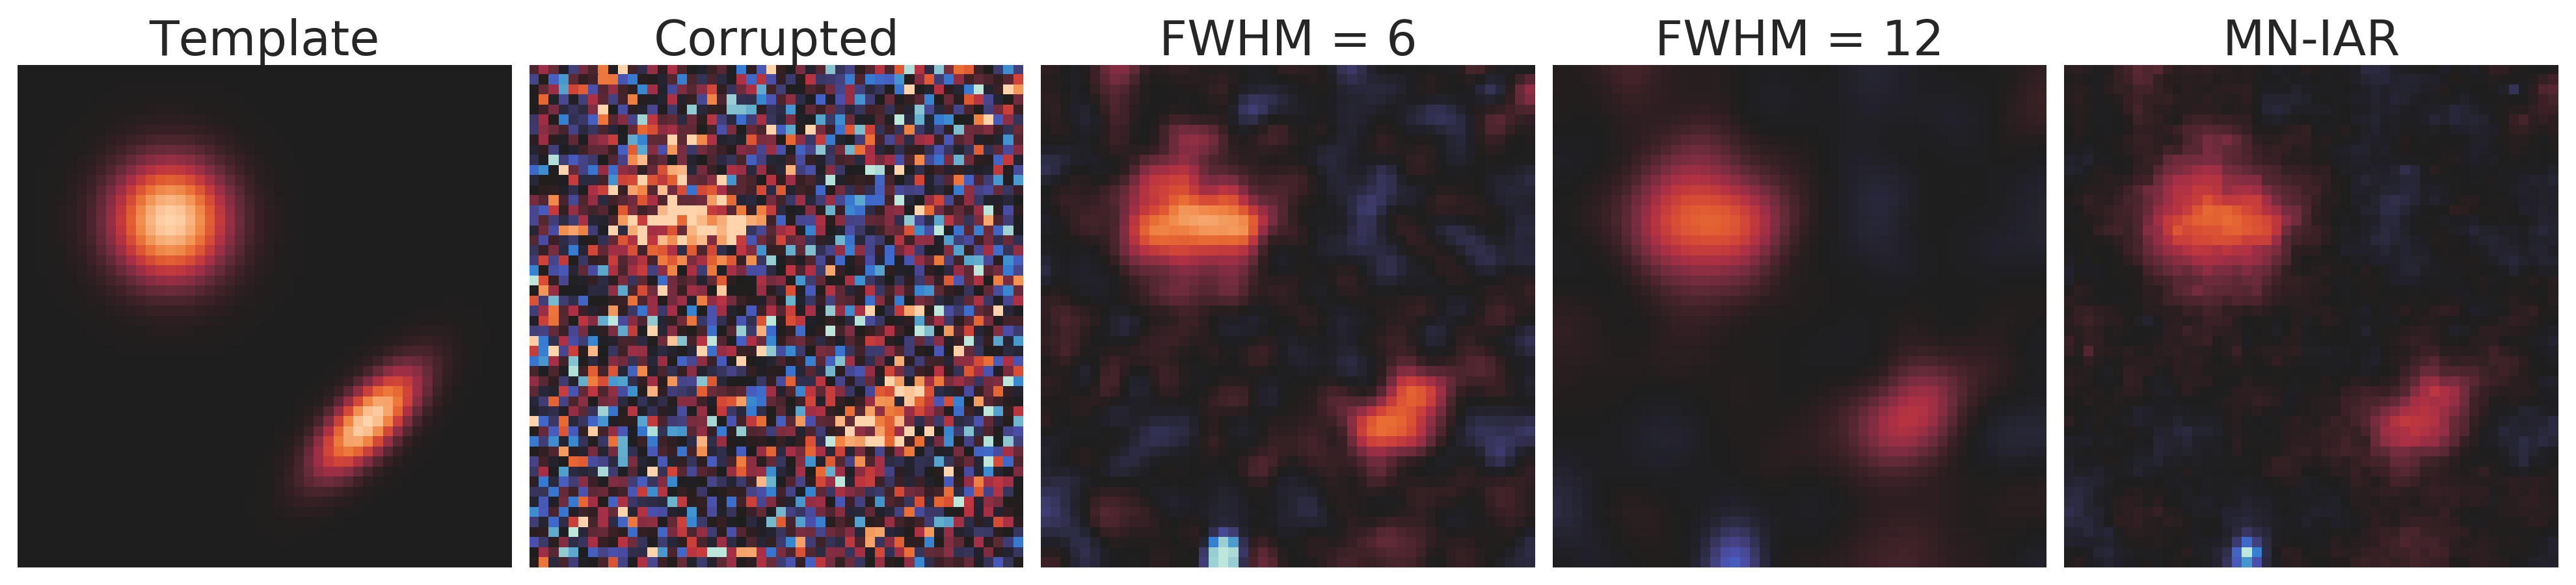
\includegraphics[trim={0 0 0 0},clip]{fig1.png}}%
}
\caption{\textbf{The Smoothing Problem for fMRI}}
\par In fMRI, the topography of latent neural activity (\textit{template}) is obscured by the presence of noise (\textit{corrupted}). As such, smoothing with a fixed-width Gaussian kernel is a common preprocessing step in fMRI analysis. Small kernels (\textit{FWHM = 6}) have the advantage of preserving signal amplitude and extent at the cost of increased false positives. Large kernels (\textit{FWHM = 12}) have the advantage of suppressing noise at the cost of blurring the image. A matrix-normal model with spatial autoregressive priors (\textit{MN-IAR}) is able to navigate this trade-off in a data-driven, spatially varying manner. 
\end{figure}

Ideally, what we would want is a smoothing method that is both data-driven (i.e. informed by the data itself) and spatially varying. Several such approaches have previously been proposed including Bayesian fMRI models with graph Laplacian priors (Penny et al., 2005; Siden et al., 2017); thin-plate spline priors (Lindquist et al., 2010); and Gaussian process priors (Harrison et al., 2008; Groves et al., 2009; Mejia et al., 2017). Here we propose a matrix-normal model for fMRI analysis with spatial priors. As will be shown, our model achieves the two properties outlined above and can be modified to incorporate any of the priors previously proposed. 

\section{Matrix Normal Models for fMRI}
Recently, Shvartsman et al. (2017) introduced matrix-normal (MN) models for fMRI analysis. The MN distribution is a generalization of the multivariate normal distribution to matrix random variables. The fMRI dataset $Y$ can be modeled as MN-distributed: 
$$ Y \sim \mathcal{MN}(XW, \Sigma_t, \Sigma_v) $$
where $Y$, $X$, and $X$ are the data, design matrix, and weights as above, and $\Sigma_t$ and $\Sigma_v$ are covariance matrices modeling the temporal and spatial structure of the data, respectively. Modeling $Y$ in this way is equivalent to the following: 
$$ \text{vec}(Y) \sim \mathcal{N}(\text{vec}(XW), \Sigma_v \otimes \Sigma_t) $$
where $\otimes$ denotes the Kronecker product of the two covariance matrices resulting in a spatiotemporal covariance matrix of size $[VT, VT]$. As discussed by Shvartsman and colleagues, the utility of the matrix-normal framework is that it allows for the simultaneous modeling of both the spatial and temporal structure of the fMRI data.

For the purposes of adaptive smoothing, the MN framework allows for the incorporation of spatial priors on the weights $W$. There are many possible choices of spatial priors, but here we focus on conditional autoregressive (CAR) priors. We select the CAR prior because it is a generalization of the graph laplacian prior already proposed for use in fMRI analysis (Penny et al., 2005; Siden et al., 2017) and because CAR priors are sparse and thus can be made to be very computational efficient. We note, however, that any of other spatial prior (e.g. thin-plate spline, Gaussian process) could be incorporated following the steps below.

To place a CAR prior on the weights, we model $W$ as MN-distributed with the properties:
$$ W_{k}^{'} \sim \mathcal{MN}(0, I, C) $$
such that the weights (across all voxels for a regressor $k$) are 0-mean with identity temporal covariance and spatial covariance $C$. The spatial covariance $C$ is equal to:
$$ C = \tau (D - \alpha A)^{-1} $$
where $D$ is a $[V,V]$ diagonal matrix whose values $d_{i,i}$ correspond to the number of neighbors for a given voxel; $A$ is the $[V,V]$ adjacency matrix where $a_{i,j} = 1$ if the voxels $i$ and $j$ are neighbors; $\tau \in R^{[0,\infty)}$ is hyperparameter scaling the magnitude of the weights; and $\alpha \in R^{(0,1)}$ is the autoregressive coefficient, determining the similarity of the weights of adjacent voxels. Importantly, when $\alpha = 1$ the prior above simplifies to $D - A = L$, or the graph Laplacian. In the following analyses we focus on this special case (also known the independent autoregressive [IAR] model) given the popularity of the graph Laplacian prior for fMRI. We note that $\alpha$ could be estimated directly from the data and we leave the effects of doing so for future study.

With the IAR prior on $W$ above, we can define the marginal-likelihood of the data $Y$ as:
$$ Y \sim \mathcal{MN}(0, \Sigma_t, C + X^T X) $$
For simplicity we will assume that the temporal covariance of the data is the scaled identity matrix, $\sigma^2 I$. In this form, we are left with two hyperparameters to estimate: $\tau$ and $\sigma$. In the following analyses we fit the MN-IAR model to both simulated and empirical data using custom software written in Python. Specifically, we make use of the \textit{scipy} optimization library (Jones et al., 2001) and the \textit{scikit-sparse} library. We exploit several programmatic tricks (Sahani and Linden 2003; Stegle et al. 2011) to avoid direct inversion of the Kronecker product of the covariance matrices during calculation of the marginal log-likelihood. As a consequence of this and the sparsity of the IAR precision matrix, fitting the MN-IAR model to an fMRI dataset of size $T=250$ and $V = 40,000$ requires less than 1 minute of computation. Thus, the MN-IAR model can scale to whole-brain fMRI without prohibitive computational demands.

\section{Results}
\subsection{Simulations}
To demonstrate the utility of the MN-IAR model, we compared its performance in recovering simulated patterns of activation against mass univariate models with three levels of smoothing: none, small kernel (FWHM = 6mm), and large kernel (FWHM = 12mm). Each simulated dataset was of 250 observations (time points) of 50x50 grid with activation magnitudes drawn from a mixture of Gaussians model. Specifically, for each dataset 2-4 activations were simulated using bivariate Gaussian kernels with centers drawn uniformly from $[5, 45]$, spatial extents drawn uniformly from $[5,25]$, and $xy$-covariance drawn uniformly from $[-0.75, 0.75]$. The max amplitude for each activation was sampled as $\mathcal{N}(2.5, 0.25)$. See Figure 1 for an example template. A timeseries dataset was then generated from each template by taking the outer product of the template with an idealized stimulus response function (i.e. boxcar function convolved with the hemodynamic response). The data were then corrupted with noise distributed $t(5,1)$ with 3 degrees of freedom. 500 total datasets of size $T=250$ and $V=2500$ were simulated.

Each model was separately fit to each simulated dataset. Model performance was compared using their sensitivity (true positive) and specificity (true negative) rates. Specifically, the signal change (weights) estimated by a model were compared against the signal change at increasing thresholds of activation. True positives were defined as when both the estimated and true signal change exceeded the threshold. True negatives were defined as when both the estimated and true signal change were beneath the threshold. The sensitivity and specificity curves for each model are presented in Figure 2. A clear trend is visible: the MN-IAR appears to compromise on the trade-off between estimation and detection power. Specifically, the MN-IAR model is more sensitive than the small kernel model (i.e. fewer false positives) and is more specific than the large kernel model (i.e. fewer false negatives). Thus, the MN-IAR model navigates the trade-off of estimation and detection power in data-driven manner: it consistently identifies the set of parameters that best preserve the signal topology and amplitude while simultaneously minimizing noise. Because the simulated data involves activations of varying spatial extent, the model is also effective for spatially-varying signals.

\begin{figure}
\centerline{%
\resizebox{1.0\textwidth}{!}{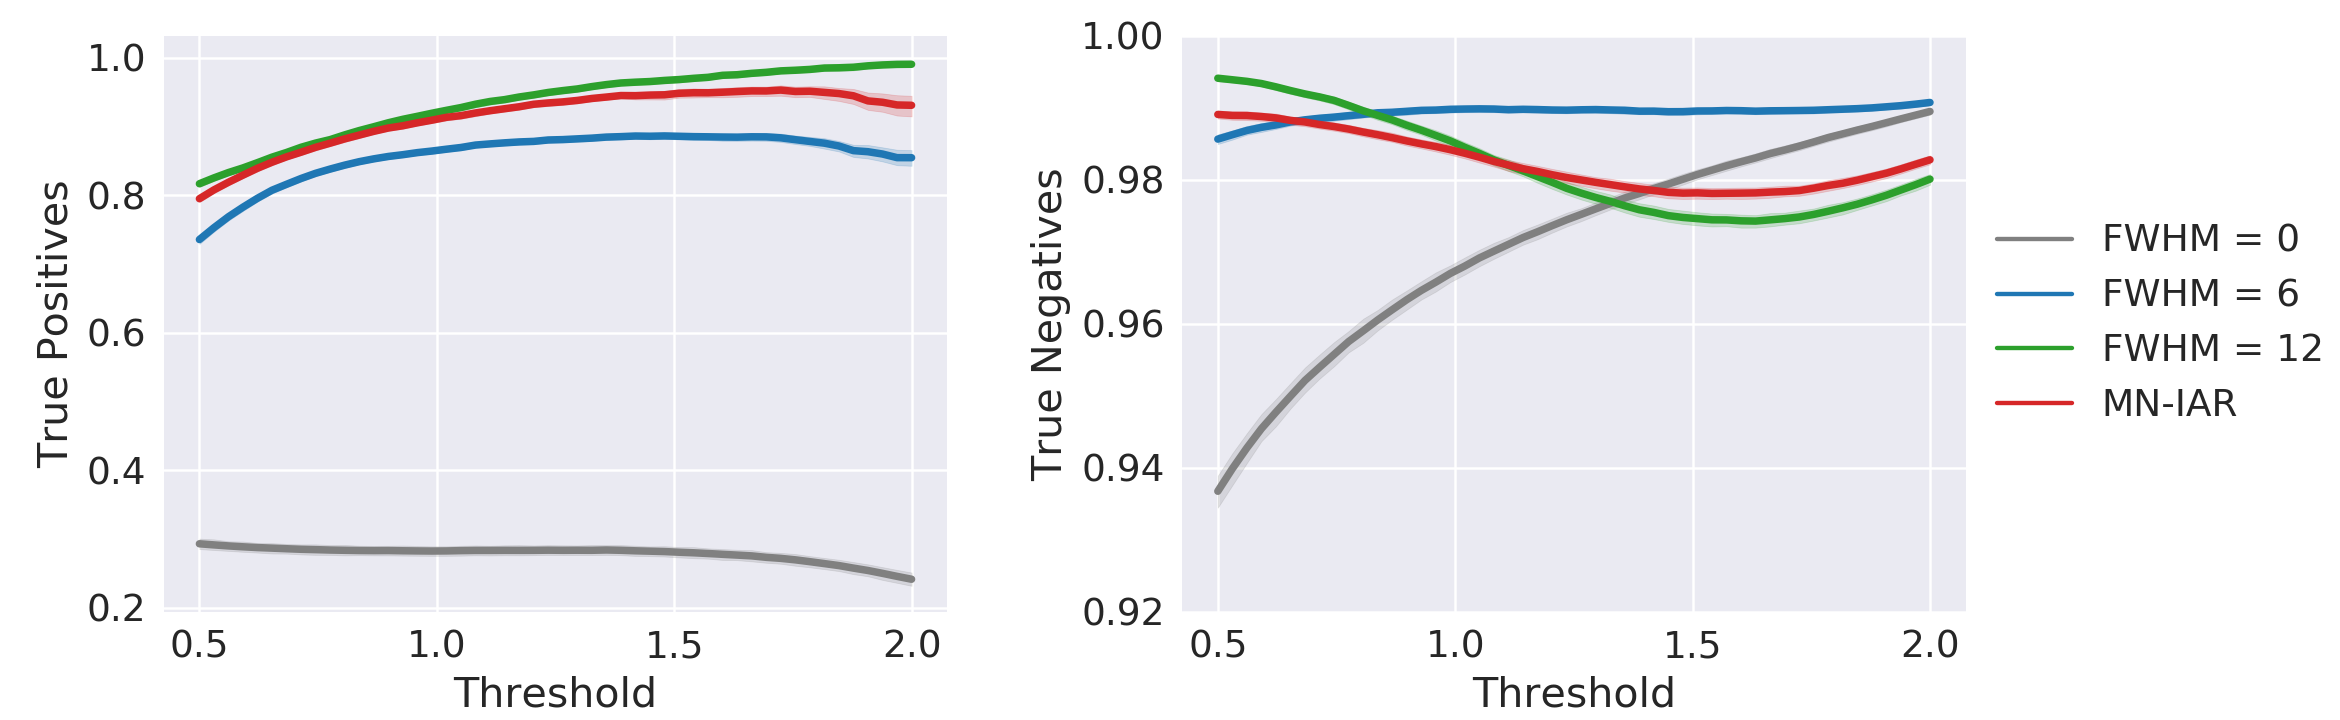
\includegraphics[trim={0 0 0 0},clip]{fig2.png}}%
}
\caption{\textbf{Comparison of Sensitivity and Specificity Curves}}
\par The true positive (sensitivity) and true negative (specificity) curves under increasing threshold levels for a no-smoothing model (FWHM = 0mm; grey), weak smoothing model (FWHM = 6mm; blue), strong smoothing model (FWHM = 12mm), and MN-IAR model (red) are presented. The MN-IAR model navigates the trade-off of estimation and detection accuracy with fewer false positives than low levels of smoothing and fewer false negatives than high levels of smoothing. All smoothing models outperform the no-smoothing model. Curves generated from 500 simulated datasets sampled from a mixtures of Gaussians model.
\end{figure}

\subsection{Empirical Data}
Next we present the performance of the MN-IAR model on real data. fMRI BOLD signal was measured in one participant during a visual stimulation task that lasted 250s (TR=1, $T=250$). The data was then preprocessed with FMRIPREP (Esteban et al., 2018) and sampled onto the Freesurfer cortical meshes (40,000 voxels per hemisphere). The data was then modeled through regression with an idealized stimulus-response regressor (i.e. boxcar function convolved with the hemodynamic response) either through least-squares with smoothing (Gaussian kernel, FWHM = 12mm) or with the MN-IAR model. 

The activation maps corresponding to the two models are presented in Figure 3. As can be observed, smoothing with a large Gaussian kernel results in a blurred activation map with one dominant peak per hemisphere (located notably in the calcarine sulcus). By contrast, the activation map corresponding to the MN-IAR is more spatially heterogeneous with multiple peak activations located across the gyri and sulci. In addition, smoothing with a large Gaussian kernel removes virtually all noise outside the visual cortex. By contrast, several (presumably spurious) activations survive thresholding for the MN-IAR model. Consistent with the simulations, we find the MN-IAR finds a set of parameters that minimizes noise while preserving topological structure. The activation maps from the MN-IAR model reveal more precise information about the locations of peak activation at the cost of increased false positives.  

A third difference between the estimates of the models is highlighted in Figure 4. Spatial smoothing with a large kernel results in considerable shrinkage of the most activated voxels. By contrast, the peak amplitudes of the MN-IAR model are greater by several percentage points. The result is that the smoothed model substantially underestimates the peak amplitude of the BOLD response to visual stimulation. Thus the MN-IAR is  more sensitive both to the topology and amplitude of the signal.
\begin{figure}
\centerline{%
\resizebox{1.0\textwidth}{!}{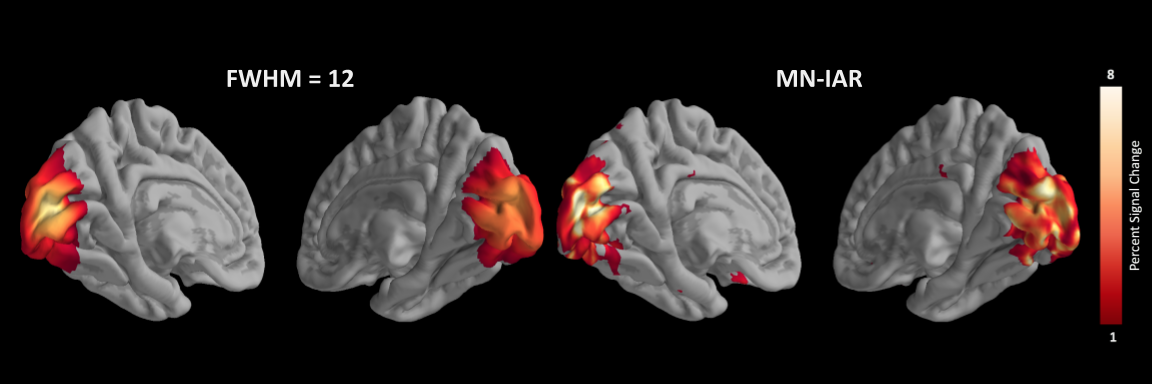
\includegraphics[trim={0 1cm 0 2cm},clip]{fig3.png}}%
}
\caption{\textbf{fMRI Activation Maps with Different Smoothing}}
\par The BOLD activation maps in response to visual stimulation in one participant from least-squares regression with fixed-width Gaussian kernel smoothing of FWHM = 12mm (left) or from MN-IAR regression (right). The MN-IAR results in smoothed activation maps that still preserve the peaks of activation across several cortical gyri/sulci. 
\end{figure}

\section{Discussion}
Conventional fMRI analysis typically involves spatial smoothing with a fixed-width Gaussian kernel. Fixed width kernels may result in increased false positives (if too small), mitigation of the signal (if too large), or both if the spatial extent of the signal is varying. Here we demonstrated the utility of matrix-normal models with spatial priors, which smooth the BOLD signal in an adaptive, data-driven manner. Specifically, we demonstrated through simulated and empirical data that the MN-IAR model finds the set of parameters that best preserves the topology and amplitude of the signal (i.e. maximizes estimation power) while reducing noise (i.e. maximizes detection power). Moreover, we showed our software to be efficient and capable of scaling to whole-brain fMRI.

Though in the present set of analyses we used an independent autoregressive (IAR) prior, we reiterate that the matrix-normal framework is flexible and amenable to any of the previously proposed spatial priors. Future research should investigate which of these may best improve estimation and detection power across different fMRI datasets. Future work on spatial priors should also investigate the use of excursion sets (Bolin and Lindgren 2015), which provide an efficient means of performing multiple comparisons corrections through the joint probabilities of sets of voxels being activated. The use of spatial priors and excursions sets may prove to be a powerful alternative to multiple comparisons corrections via the standard approach using Gaussian Markov random fields, which have been shown to frequently yield high false positive rates (Eklund et al. 2016).

\begin{figure}
\centerline{%
\resizebox{1.0\textwidth}{!}{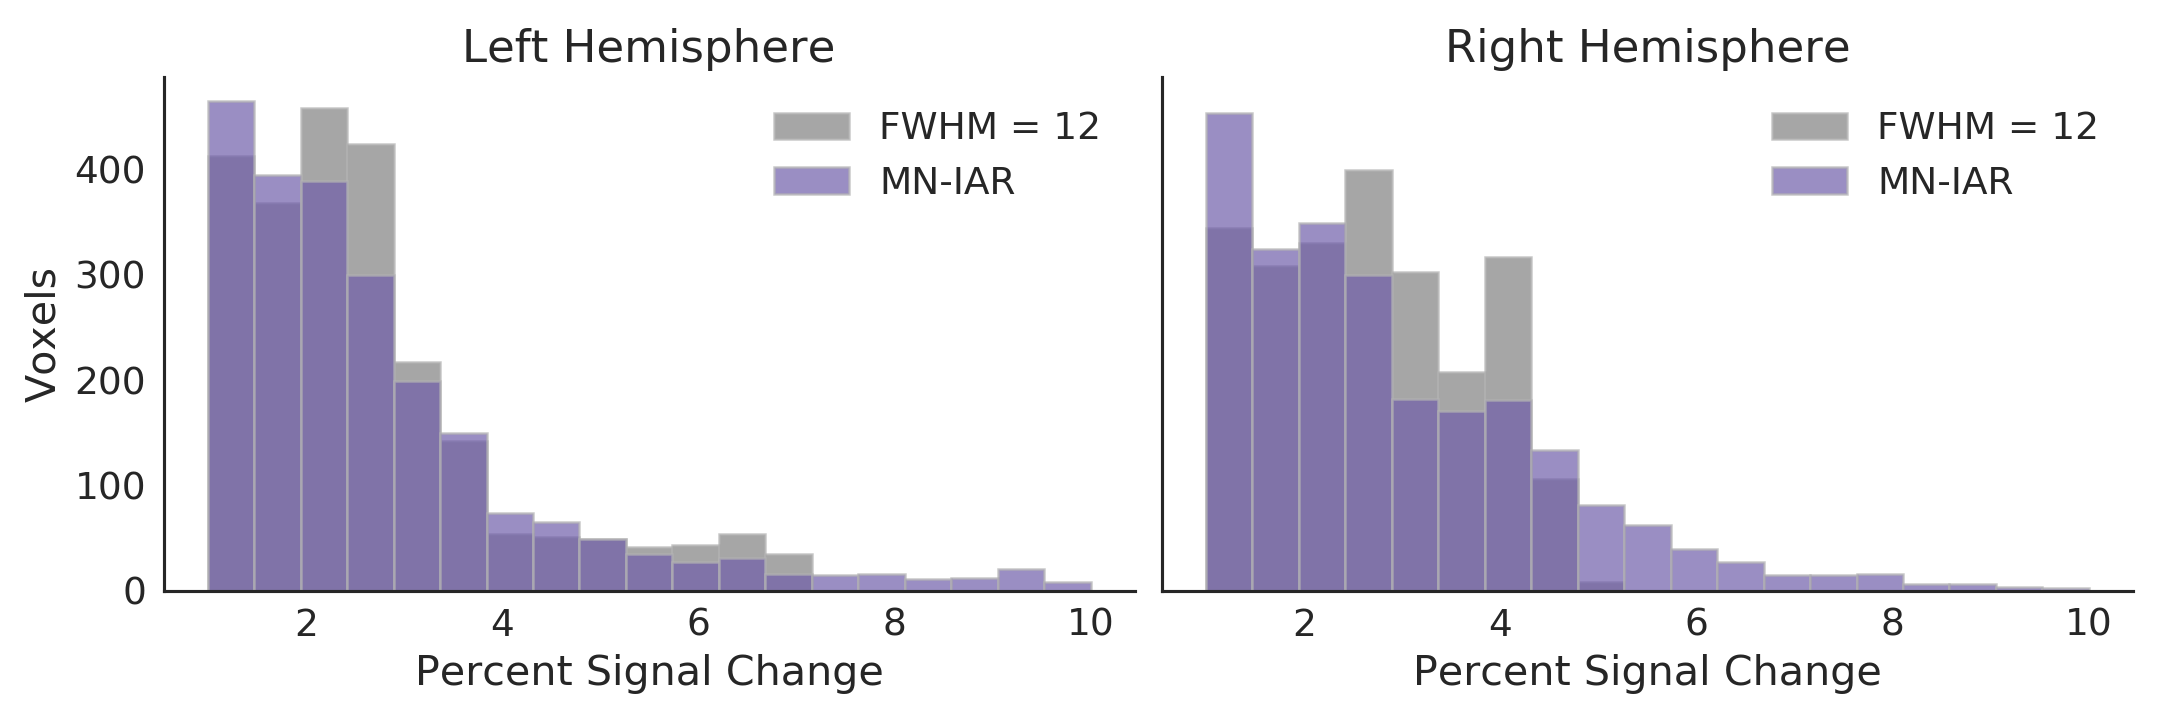
\includegraphics[trim={0 0 0 0},clip]{fig4.png}}%
}
\caption{\textbf{Comparison of Estimated BOLD Change across Voxels}}
\par The estimated BOLD response to visual stimulation in one participant from either least-squares regression with fixed-width Gaussian kernel smoothing of FWHM = 12mm (grey) or from MN-IAR regression (purple). Smoothing with large kernels results in the shrinkage of the most activated voxels. By contrast, the MN-IAR model preserves the signal amplitude of the most activated voxels. 
\end{figure}

\nocite{*} 
\bibliography{NEU560-final}

\end{document}